\chapter{Results} \label{sec:results}

\section{Beluga simulation}

\subsection{Introduction}
\par In order to evaluate the differences between variational inference techniques (ADVI, BBVI, SVGD) and MCMC, we generate a simulated dataset where the true values are known. Doing so, it becomes possible to check not only that the different techniques reach the same final results, but also whether any inference method actually correctly estimates the ground truth.
\medskip
\par First we study the inference of the duplication ($\bm\lambda$) and loss ($\bm\mu$) rates for each species tree branch. Note that there is also a global parameter $\eta$ (which models the probability of a multiple ancestral genes at the root) for the whole tree that has to be inferred. The species tree used in this experiment contains nine plant species (see Figure \ref{fig:plants-tree}). Because this experiment is a simulation, this will be the only time in this chapter where we have access to ground truth values.

\subsection{Beluga simulation}

A Beluga model with a certain set of parameters ($\bm\lambda$, $\bm\mu$, $\eta$) was created and used to generate 500 simulated samples of gene counts. These were then randomly subsampled into mini-batches of 200 samples for the variational inference methods, while MCMC used the full dataset each iteration.
\medskip
For this simulation the inference algorithms are set up up as follows:
\begin{itemize}
    \item ADVI uses 1 MC sample and mini-batches of 200 samples. The algorithm is run for 1000 iterations.
    \item BBVI uses 10 MC samples and mini-batches of 200 samples. The algorithm is run for 1000 iterations. The variational family used here is the same mean-field distribution as used in ADVI.
    \item MCMC is run for 5000 iterations, of which 1000 are burn-in samples
    \item SVGD uses 50 particles and is run for 500 iterations with mini-batches of 50 samples.
\end{itemize}

\begin{figure}
	\centering
	\includegraphics[width=7in]{images/trees/plants-tree.png}
	\caption[Species tree for simulated plant data.]{Species tree for the plant species in the Beluga simulation study.}
    \label{fig:plants-tree}
\end{figure}


\subsubsection{Comparison of VI convergence}
Before comparing variational inference with MCMC, the optimisation of the different variational algorithms can be compared. The convergence process of the various model parameters are shown in Figures \ref{fig:beluga-sim-opt-lambda} and \ref{fig:beluga-sim-opt-mu}. It is clear that both ADVI and BBVI algorithms do not converge to the ground truth values in all cases, but we shall see that the more accurate MCMC algorithm also doesn't exactly find all of the parameters.

\medskip
\par When plotting the progress of the ELBO function, it is clear that BBVI converges faster than ADVI. While the BBVI gradient estimator is more noisy than ADVI, the rolling average of the ELBO that is shown in Figure \ref{fig:score} appears no more noisy than that of ADVI.

\begin{figure}
	\centering
	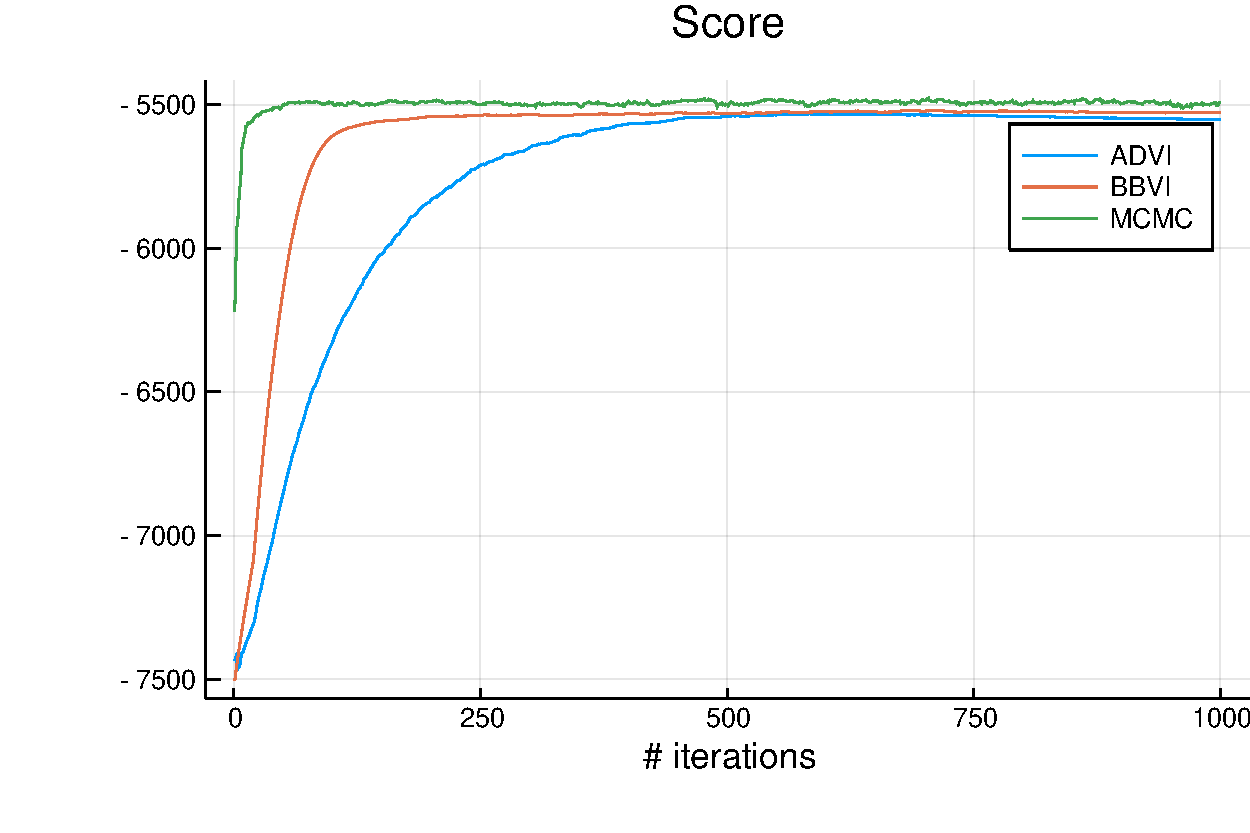
\includegraphics[width=4in]{images/simulations/beluga-sim-score.pdf}
	\caption[Beluga simulation: VI optimisation comparison]{Comparison of score functions between VI methods ADVI and BBVI, which use the ELBO as score (rolling average over 20 iterations), and the MCMC, which uses the joint likelihood. because they use different score functions the VI methods cannot be directly compared to the MCMC.}    
	\label{fig:score}
\end{figure}

\begin{figure}
	\centering
	\noindent\makebox[\textwidth]{
	    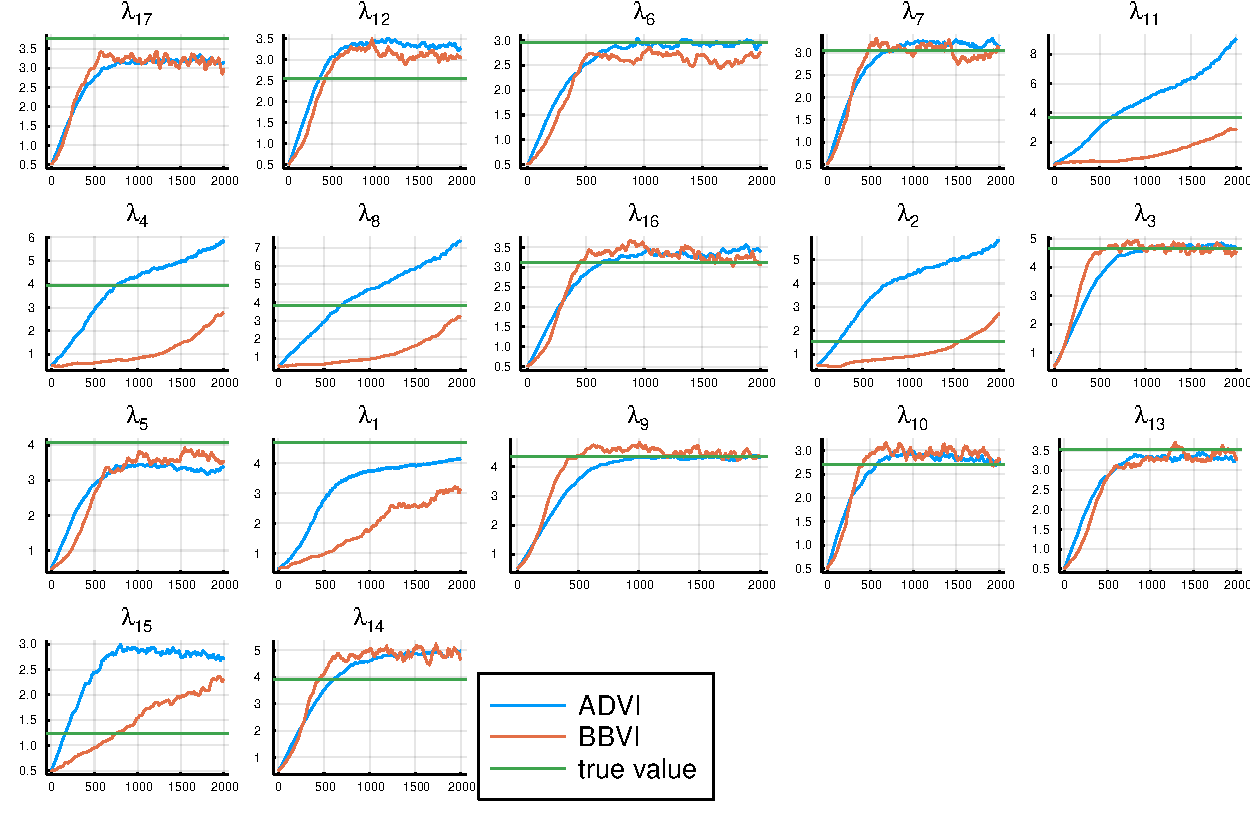
\includegraphics[width=7.5in]{images/simulations/convergence-lambda.pdf}
    }
	\caption[Beluga simulation: VI optimisation comparison for $\lambda$.]{Plots of the variational optimisation process of the variational parameter $\bm\mu$ which models the duplication rates $\bm\lambda$. Each plot shows the duplication rate for a different branch in the species tree. Both BBVI (red) and ADVI (blue) are shown in relation to the ground truth values (green).}
    \label{fig:beluga-sim-opt-lambda}
\end{figure}

\begin{figure}
	\centering
	\noindent\makebox[\textwidth]{
	    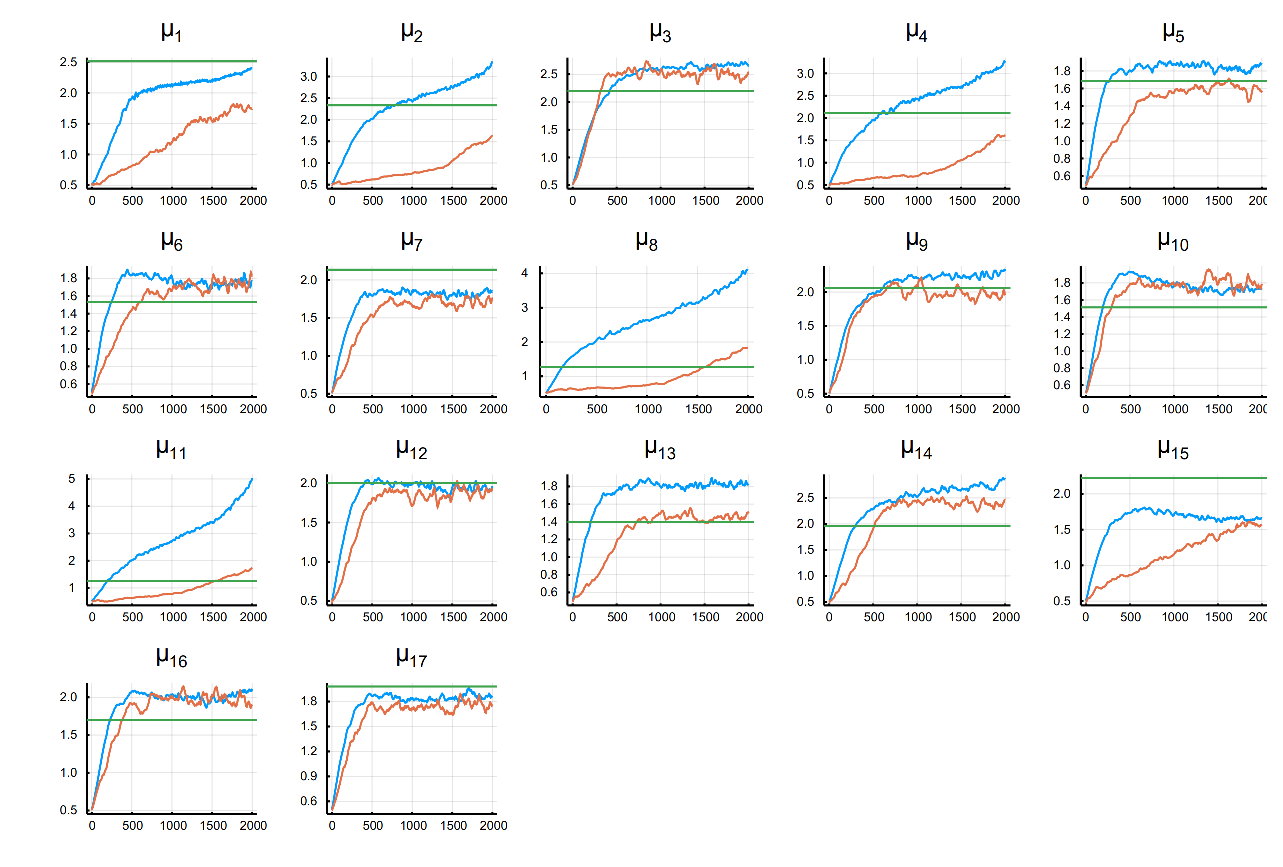
\includegraphics[width=7.5in]{images/simulations/convergence-mu.eps}
	}
	\caption[Beluga simulation: VI optimisation comparison for $\mu$.]{Plots of the variational optimisation process of the variational parameter $\bm\mu$ which models the loss rates $\bm\mu$. Each plot shows the loss rate for a different branch in the species tree. Both BBVI (red) and ADVI (blue) are shown in relation to the ground truth values (green).}
    \label{fig:beluga-sim-opt-mu}
\end{figure}


\subsubsection{Comparison with MCMC}
The approximate VI distributions for each latent model parameter can be compared to the distribution of the MCMC trace (Figures \ref{fig:beluga-sim-distribution-lambda}, \ref{fig:beluga-sim-distribution-mu}). It is immediately evident from the figures that none of the methods find the all the correct parameter values, not even MCMC which is expected to be the most accurate.
\\
While both VI methods provide reasonable approximations, it is clear that the variational distribution of BBVI (blue in Figures \ref{fig:beluga-sim-distribution-lambda} and \ref{fig:beluga-sim-distribution-mu}) more exactly matches the posterior found by MCMC. While ADVI has a very similar mean, the distribution is often too narrow. In practice we notice that the variational parameters for the variance ($\bm\omega$) of ADVI do not change much from the starting values, so a correct initial estimate is paramount; BBVI suffers from the same problem to a lesser extent.
\\
SVGD (with 50 particles) is plotted separately against MCMC to avoid cluttering in the plot (see Figure \ref{fig:beluga-sim-svgd}). We provide only the duplication rates here because this is sufficient to see that SVGD does not provide anywhere near the accuracy of BBVI or ADVI; there are several branches where the algorithm completely misses the target which does not happen with the other two VI methods.



\begin{figure}
    \noindent\makebox[\textwidth]{
	    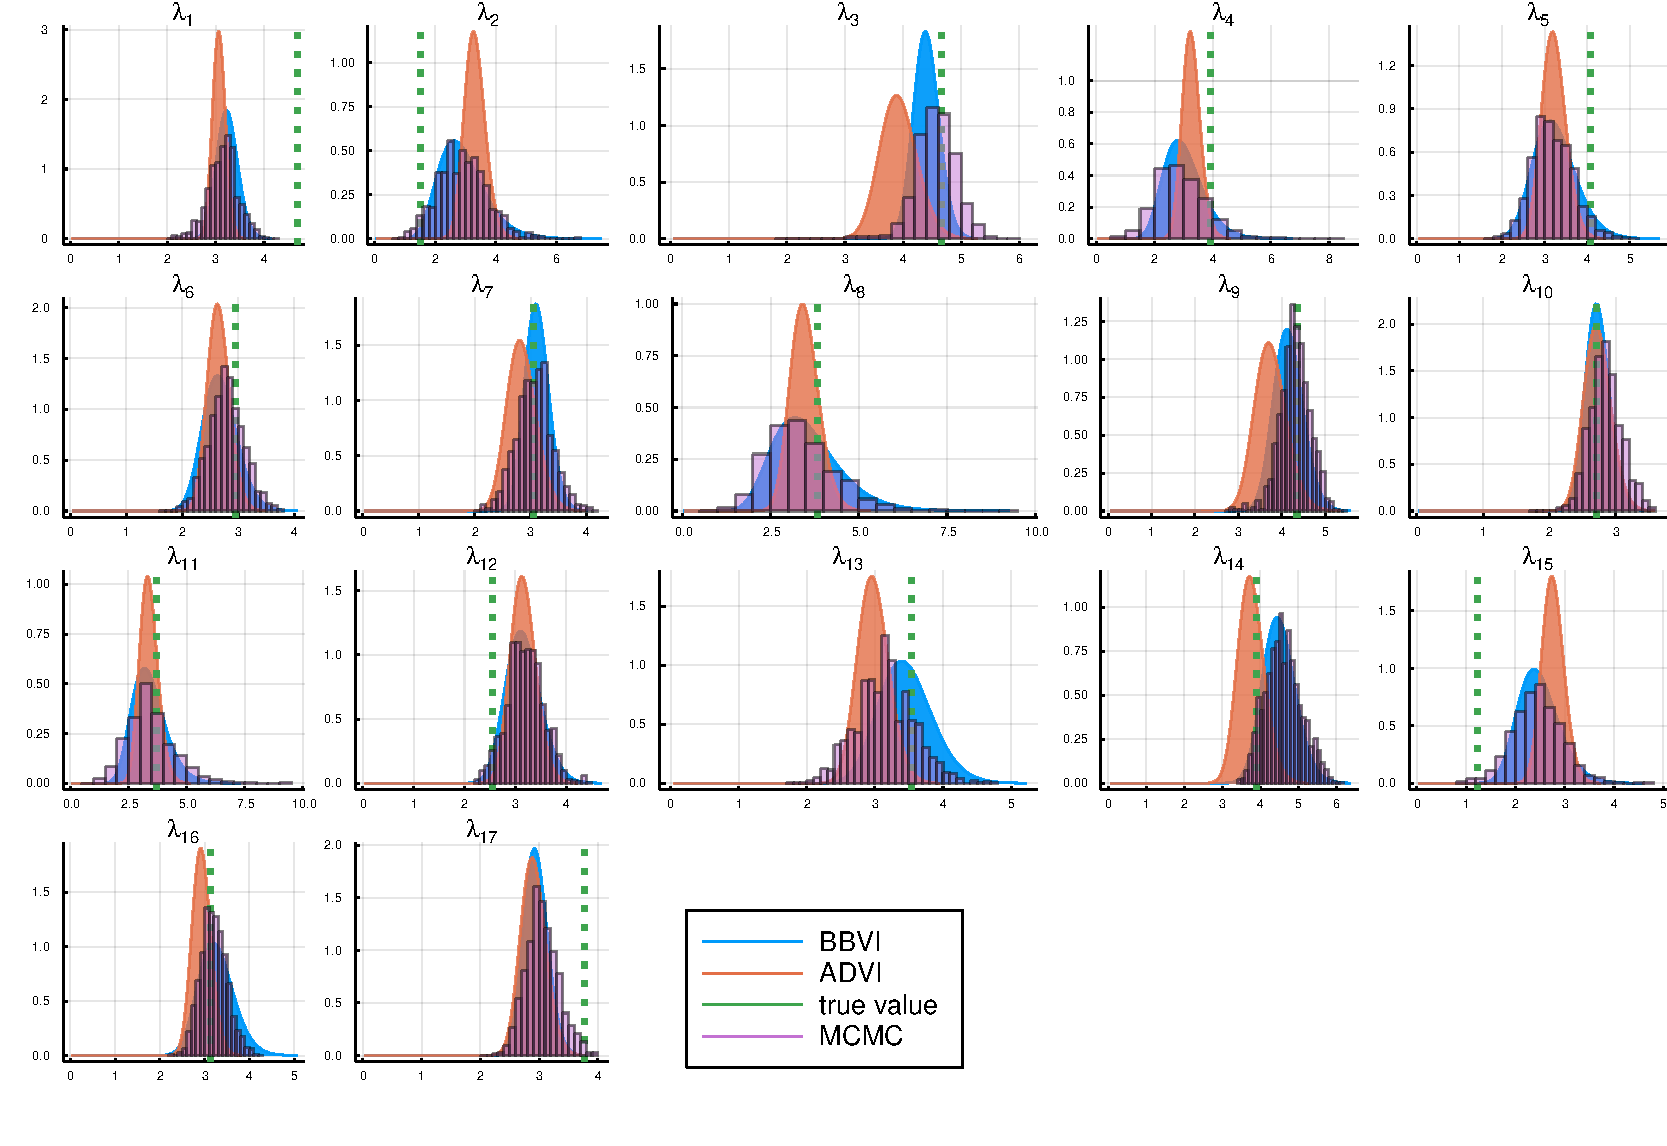
\includegraphics[width=7in]{images/simulations/beluga-sim-distribution-lambda.pdf}
	}
	\caption[Beluga simulation: VI approximation and MCMC comparison]{A comparison of the variational approximations and MCMC for the $\lambda$ parameters of the Beluga model on a simulated dataset. The approximations for ADVI (orange), BBVI (blue) are compared with MCMC (pink) and the ground truth values of the simulation (green).}
    \label{fig:beluga-sim-distribution-lambda}
\end{figure}

\begin{figure}
    \noindent\makebox[\textwidth]{
	    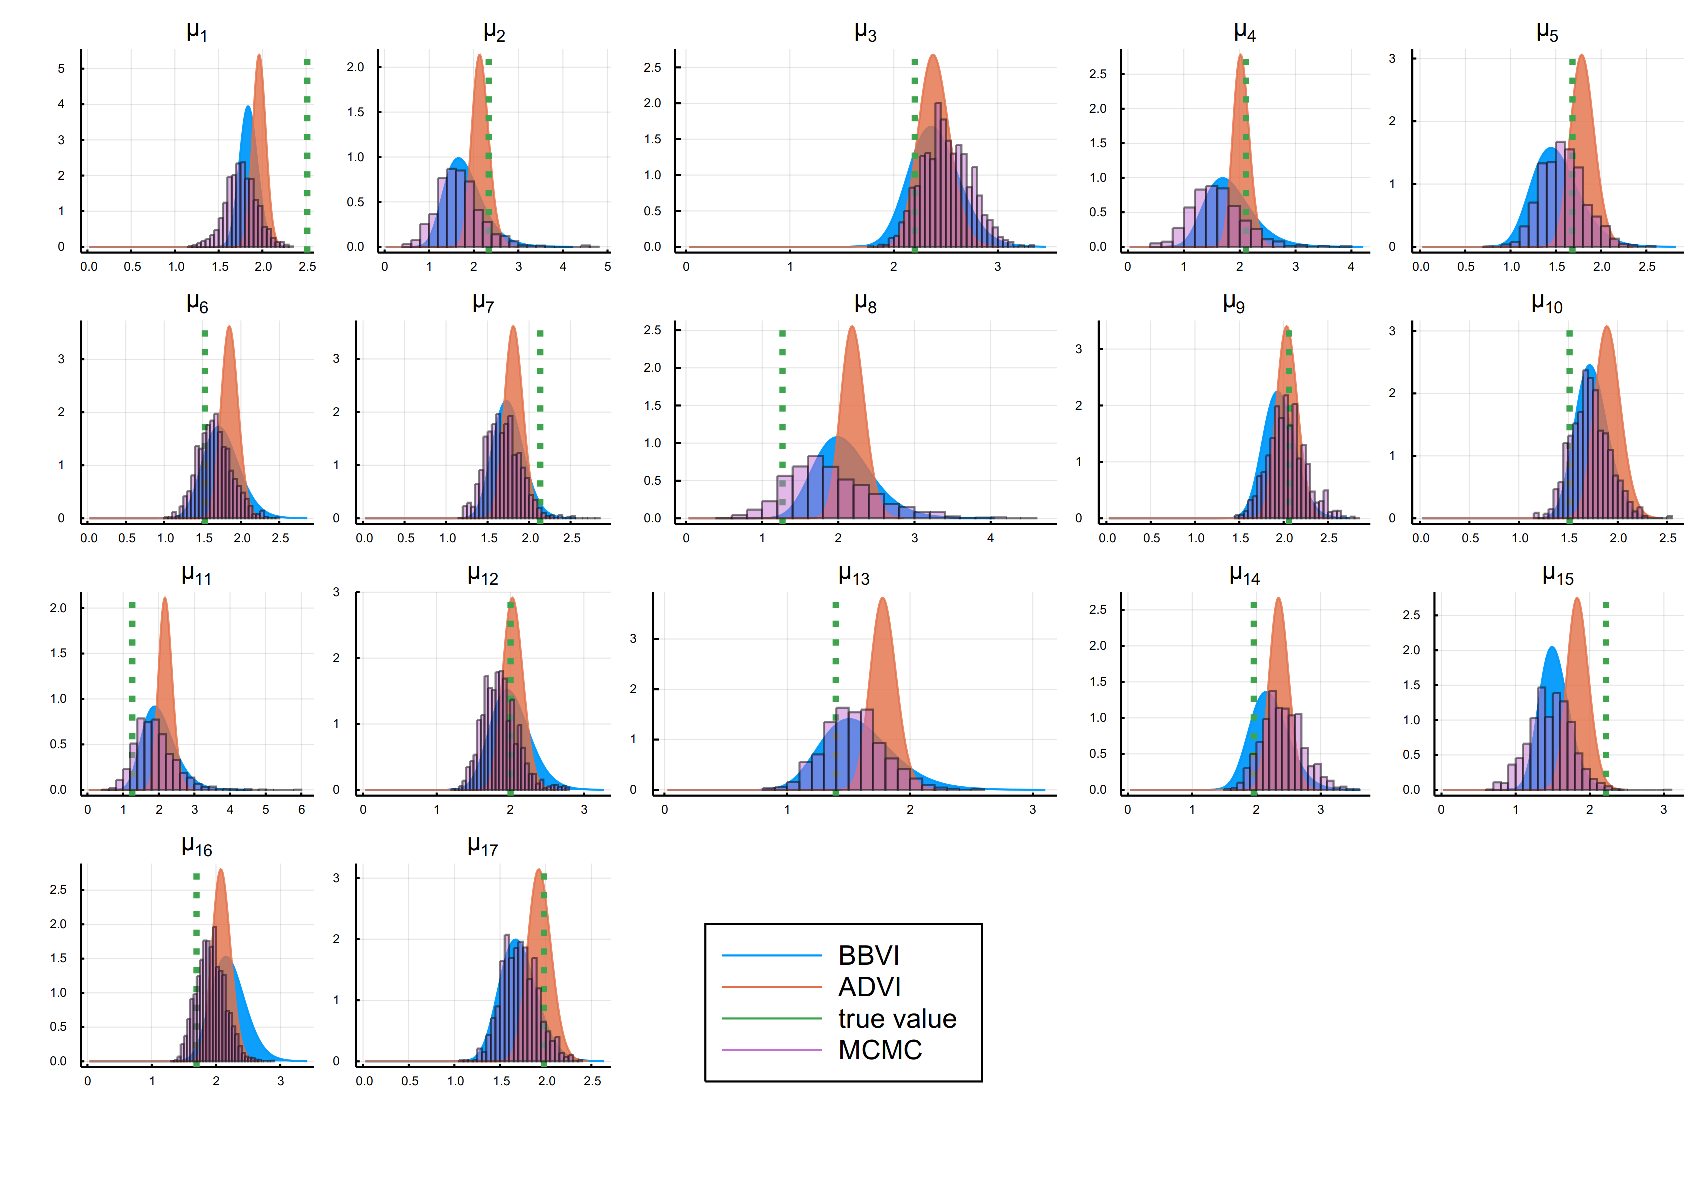
\includegraphics[width=7in]{images/simulations/beluga-sim-distribution-mu.eps}
	}
	\caption[Beluga simulation: VI approximation and MCMC comparison]{A comparison of the variational approximations and MCMC for the $\mu$ parameters of the Beluga model on a simulated dataset. The approximations for ADVI (orange), BBVI (blue) are compared with MCMC (pink) and the ground truth values of the simulation (green).}
    \label{fig:beluga-sim-distribution-mu}
\end{figure}

\begin{figure}
    \noindent\makebox[\textwidth]{
	    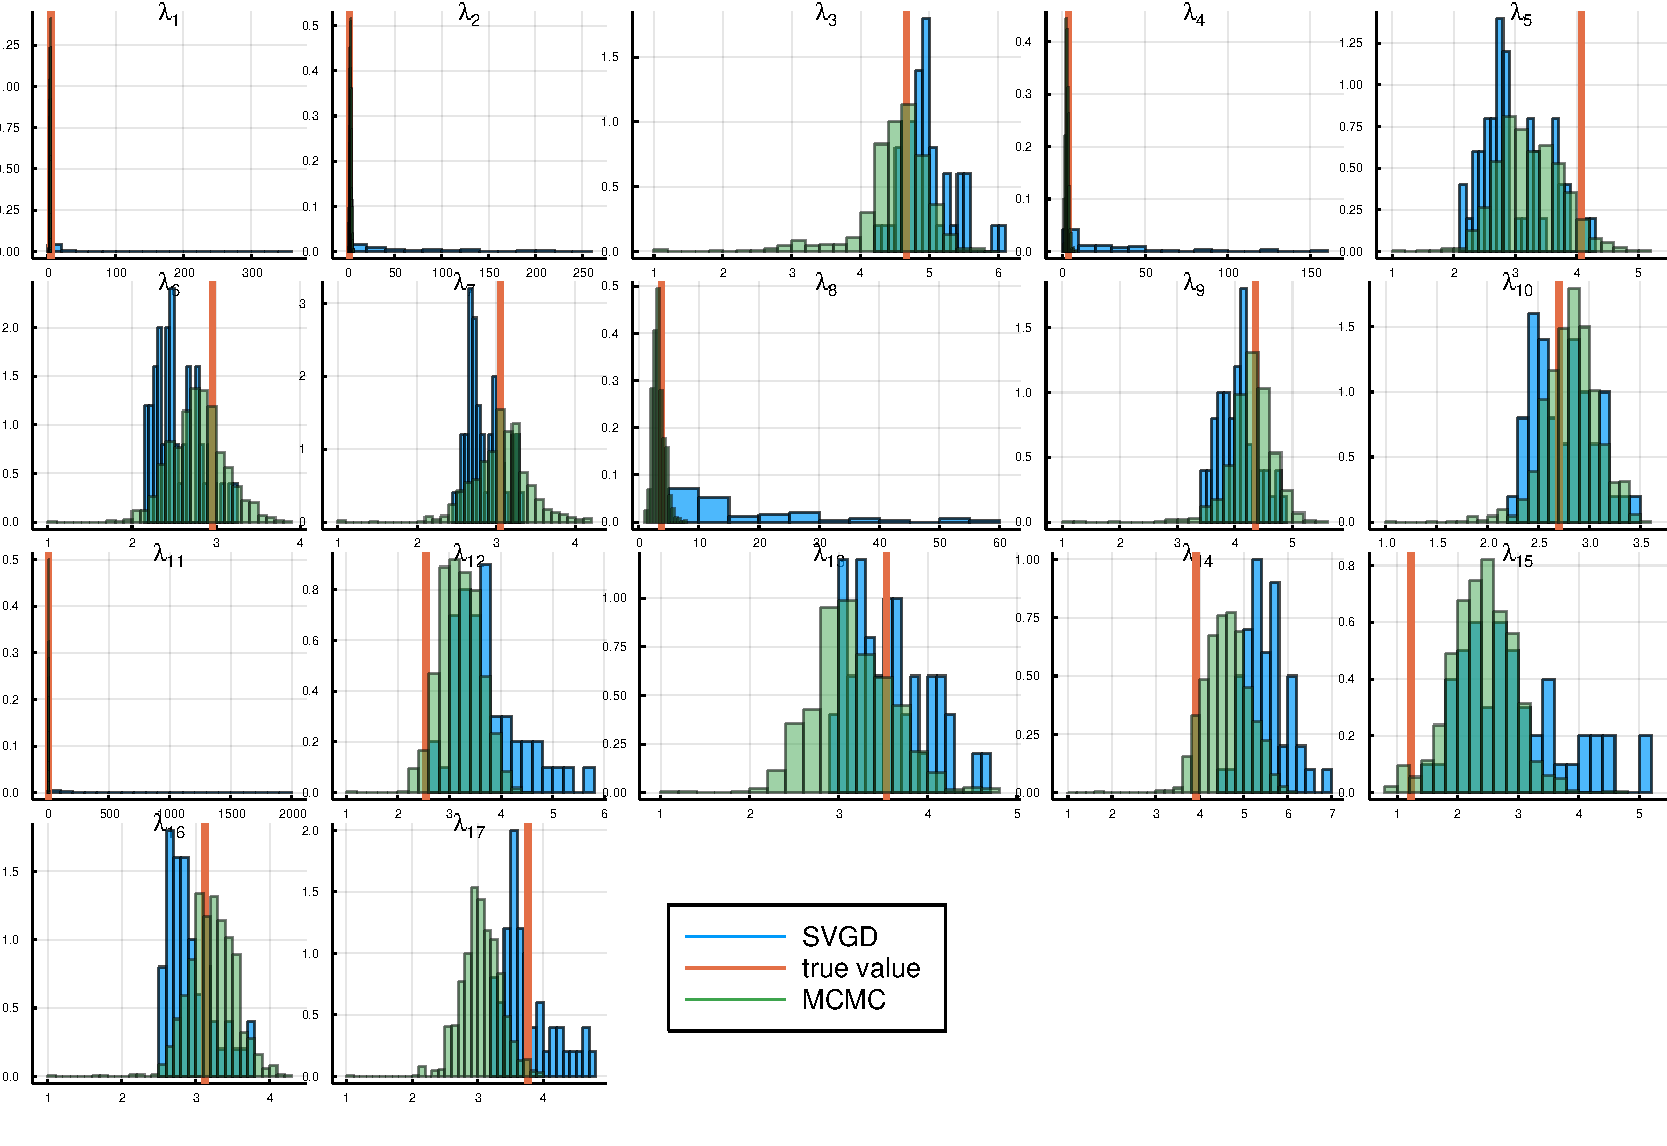
\includegraphics[width=7in]{images/simulations/beluga-sim-distribution-mu.pdf}
	}
	\caption[Beluga simulation: VI approximation and MCMC comparison]{A comparison of the variational approximations and MCMC for the $\lambda$ parameters of the Beluga model on a simulated dataset. The approximations for ADVI (orange), BBVI (blue) are compared with MCMC (pink) and the ground truth values of the simulation (green).}
    \label{fig:beluga-sim-svgd}
\end{figure}

\subsubsection{Time analysis}
While variational inference is known to be less accurate than MCMC - it is always an approximate solution - the advantage of VI cited in the literature \parencite{vi-review} is that it is faster. Our simulation experiment confirms this: both VI methods are indeed considerably faster. Among the different variational methods tested, BBVI is clearly the fastest. 
\\
This is likely because the models studied in this thesis have very expensive model gradients, which means that the methods which use this gradient (ADVI, SVGD) are at a disadvantage here when it comes to computational time. These methods will be more competitive when the model gradient $\nabla\mathrm{log}p(\bm x, \bm\theta)$ is not much more expensive than the model density $\mathrm{log}p(\bm x, \bm\theta)$ as is the case here.
\\
SVGD typically uses at least 50 particles, which in this case would be much slower than the MCMC. For being slower than the gold standard, we will discard SVGD in the rest of the experiments in this chapter and only continue comparing ADVI, BBVI and MCMC.



\begin{table}[]

    \caption[Beluga computation time benchmarks]{Computation time benchmarks for the Beluga simulation data. ADVI and BBVI use 1 and 10 Monte Carlo samples respectively, and al VI methods use mini-batches of 100 samples. A full analysis consists of 1000 iterations for ADVI, SVGD and BBVI, and 5000 iterations for MCMC.}
    \centering
    \begin{tabular}{l||lllll|}
    \cline{2-5}
     & \multicolumn{4}{c|}{\textbf{Inference method}}                                                                            \\ \hline
    \multicolumn{1}{|l||}{\textbf{\# iterations}} & \multicolumn{1}{l|}{ADVI} & \multicolumn{1}{l|}{BBVI}  & \multicolumn{1}{l|}{SVGD-50} & MCMC \\ \hline
    \multicolumn{1}{|l||}{1}                      &         1.08s             &          \textbf{0.48s}               &            3.83s                 &                                 0.56s   \\ \hline
    \multicolumn{1}{|l||}{10}                     &         11.52s            &           \textbf{4.12s}                &          43.1s           &                       6.70s \\ \hline
    \multicolumn{1}{|l||}{full analysis}          &         1103.2s                  &     \textbf{389.9s}         &     4074.95s                &                                 3476.9s   \\ \hline
    \end{tabular}
    \label{tab:time-sim}

\end{table}


\section{Beluga with real-world data}

\par The previous section described a comparison of the variational approaches with traditional MCMC sampling on a synthetic dataset generated with the Beluga model. This section contains similar comparisons but for problems with real-world datasets. 


\subsection{Beluga rice dataset}

\par Now we present a study of the phylogenetic relationship between more closely related plant species. High-quality gene count data is available for different species of rice which have a common ancestor estimated at $\sim$15 Mya. A species tree is reconstructed from a figure available in the original paper (\cite{rice}, Figure 1.b), where \textit{L. perrieri} is added as an outgroup to the rice species. Since these species are very closely related, we do not expect much activity in the branches. Both the duplication and loss rates should be small.

\begin{comment}
Because the rice species are closely related, we do not expect to find evidence of a whole genome duplication event within the rice. It is, however, widely accepted that a WGD event occurred shortly before the speciation event in the common ancestor of rice ($\sim$20 Mya) \parencite{rice-split}.
\end{comment}

\begin{comment}
\subsubsection{Preprocessing}
Gene families that did not have at least one gene in the \textit{L. perrieri} branch were filtered out. Typically gene families are also further filtered on size as extremely large and extremely small families are removed from the data.
\end{comment}

\subsubsection{Results analysis}
It is very clear in this case that VI is much faster: running the MCMC algorithm for 10,000 iterations (of which 1000 burn-in) takes several hours (430.8 min), while the ADVI and BBVI algorithms converge in less than an hour (30.2 min and 23.8 min respectively).
\medskip
\par The results are similar to the simulation study, in that we find BBVI to be most like the MCMC results, with ADVI showing results that deviate somewhat more. We find that many branches have duplication and loss rates that are nearly zero, which is expected since these rice species are all close relatives.

\begin{figure}
	\centering
	\includegraphics[width=6.5in]{images/trees/rice-species-tree.png}
	\caption[Species tree of rice dataset]{Species tree of the rice dataset, containing 10 species of rice and \textit{Leersia perrieri} as an outgroup. Also see Figure 1.b in Stein et al. \parencite{rice}.}
    \label{fig:rice-tree}
\end{figure}

\begin{figure}
    \noindent\makebox[\textwidth]{
	    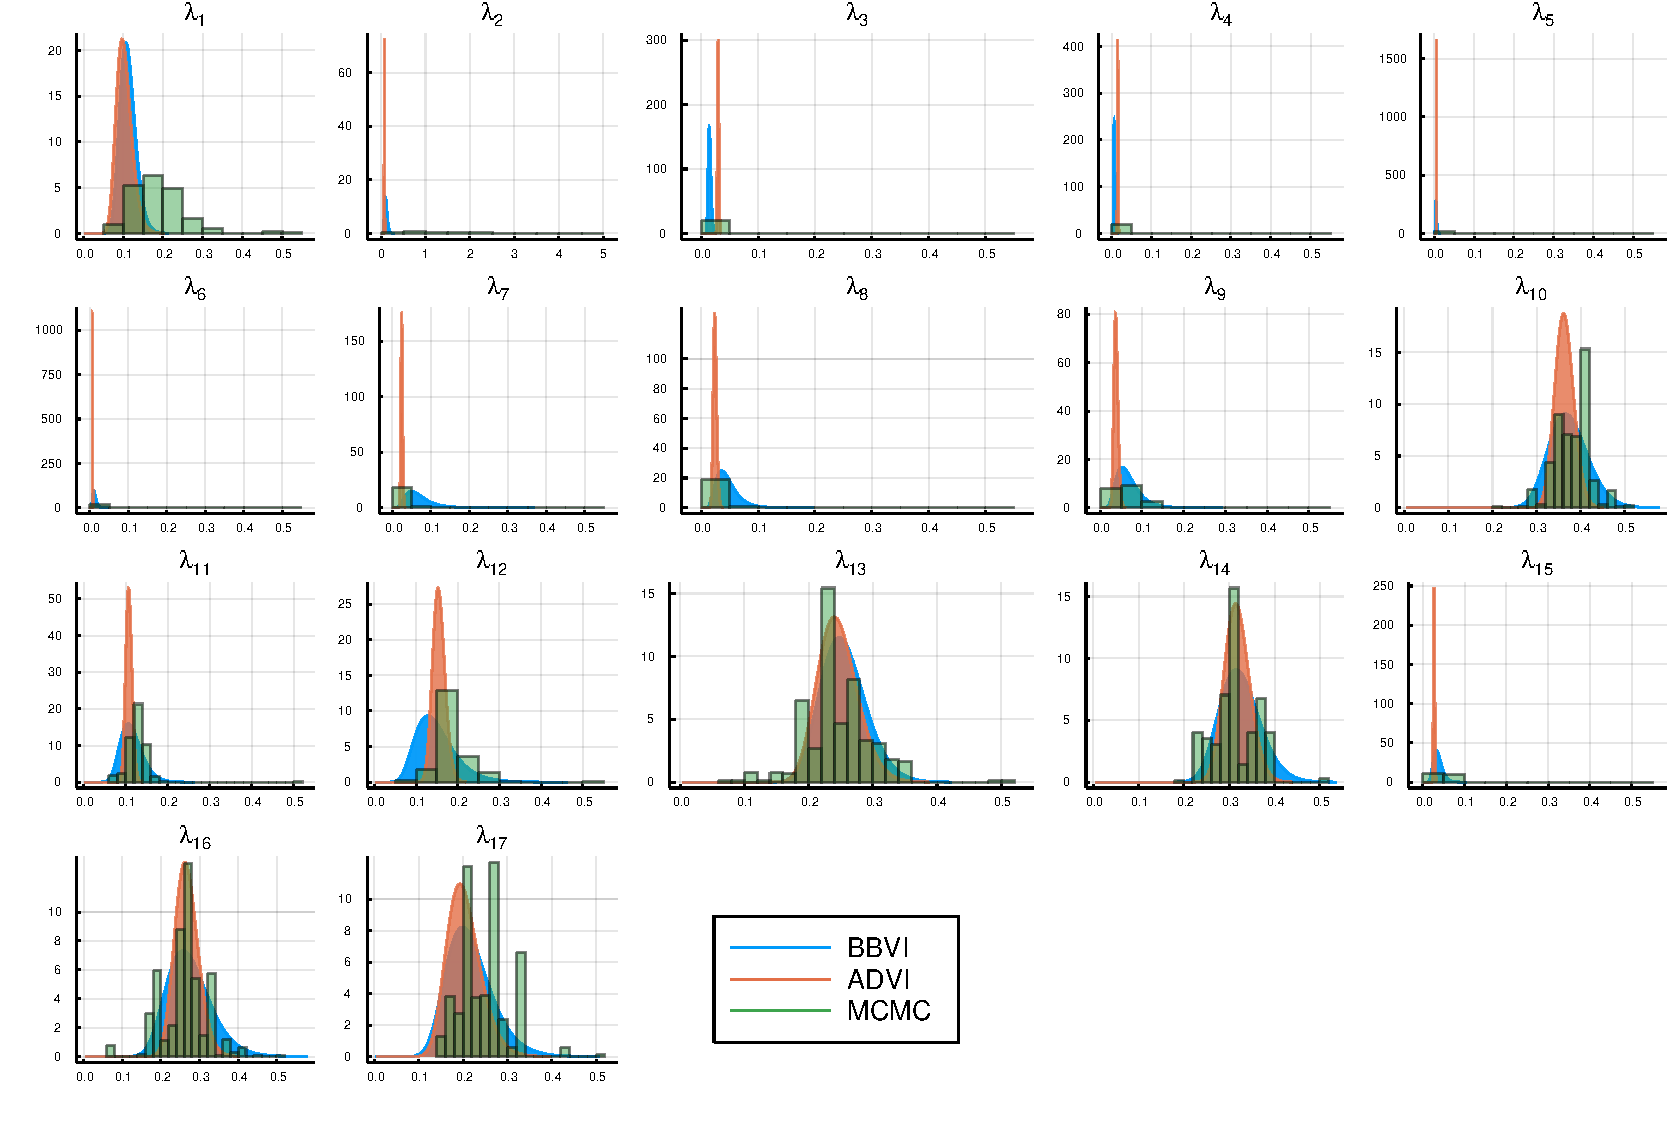
\includegraphics[width=7.2in]{images/rice/rice-lambda.pdf}
	}
	\caption[Rice Beluga duplication rates]{Overview of the distributions of the duplication rates $\lambda$ in each branch for the Beluga analysis of the rice dataset.}
    \label{fig:rice-lambda}
\end{figure}

\begin{figure}
    \noindent\makebox[\textwidth]{
	    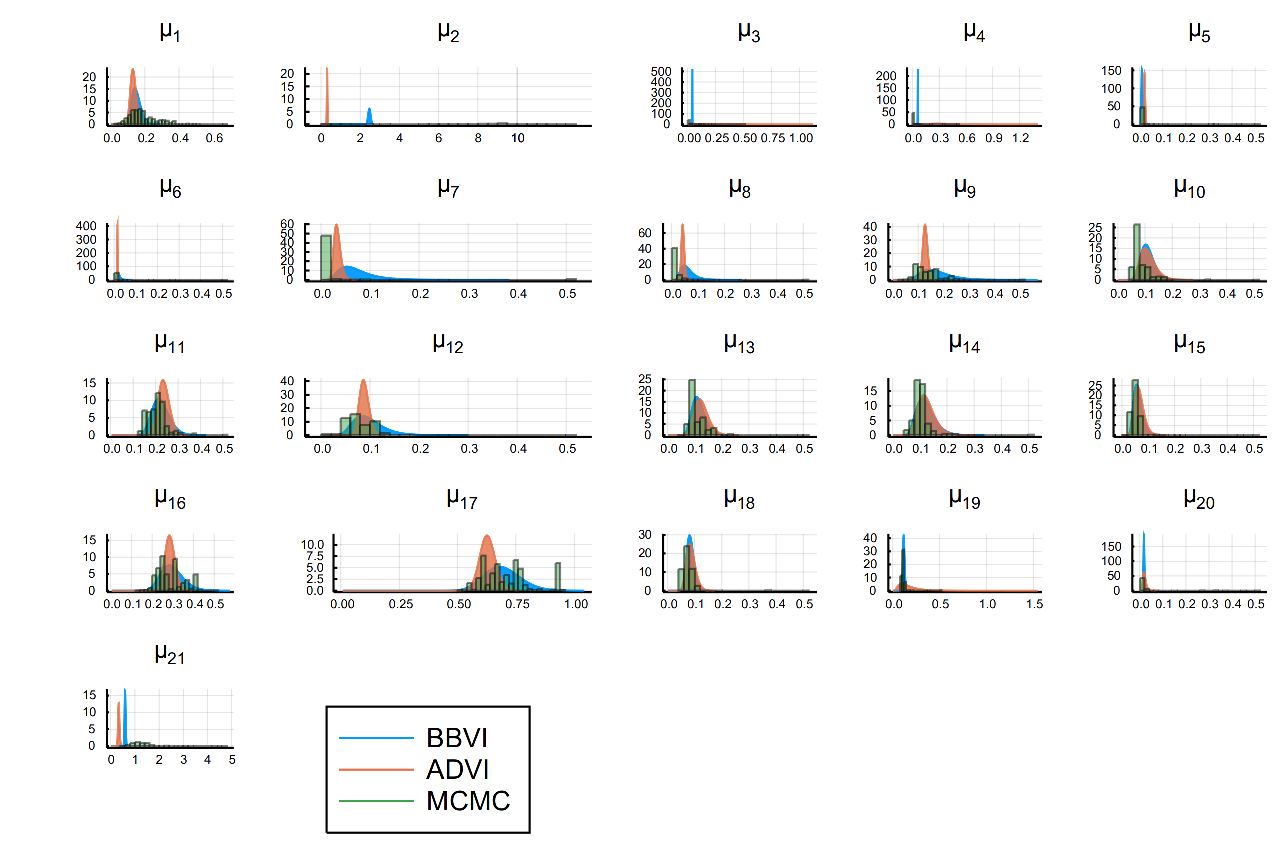
\includegraphics[width=7.2in]{images/rice/rice-mu.eps}
	}
	\caption[Rice Beluga duplication rates]{Overview of the distributions of the loss rates $\mu$ in each branch for the Beluga analysis of the rice dataset.}
    \label{fig:rice-lambda}
\end{figure}


\subsection{Beluga PLAZA dataset}

\par The PLAZA access platform \parencite{PLAZA-paper-1, PLAZA-paper-2} contains a curated set of genomic and transcriptomic data compiled from different sequencing studies. In this thesis we use a subset of the PLAZA 4.0 dicot dataset which contains 44 plant species (Figure \ref{fig:PLAZA-trees}).
\medskip
\par The PLAZA dataset is an example of a problem that cannot feasibly be solved with the existing MCMC method because it would take too long to compute. For 44 species the Beluga model contains 89 duplication rates, 89 loss rates and an additional parameter $\eta$. Variational methods are useful here because they can operate on small mini-batches of data instead of the full dataset. For computational reasons only 250 gene families were used here. BBVI was the only method tested here because it is the only method that reached a stable result; ADVI would collapse into a situation with infinite variance which crashed the optimisation process.

\begin{figure}
    \noindent\makebox[\textwidth]{
        \hspace{-2.6cm}
	    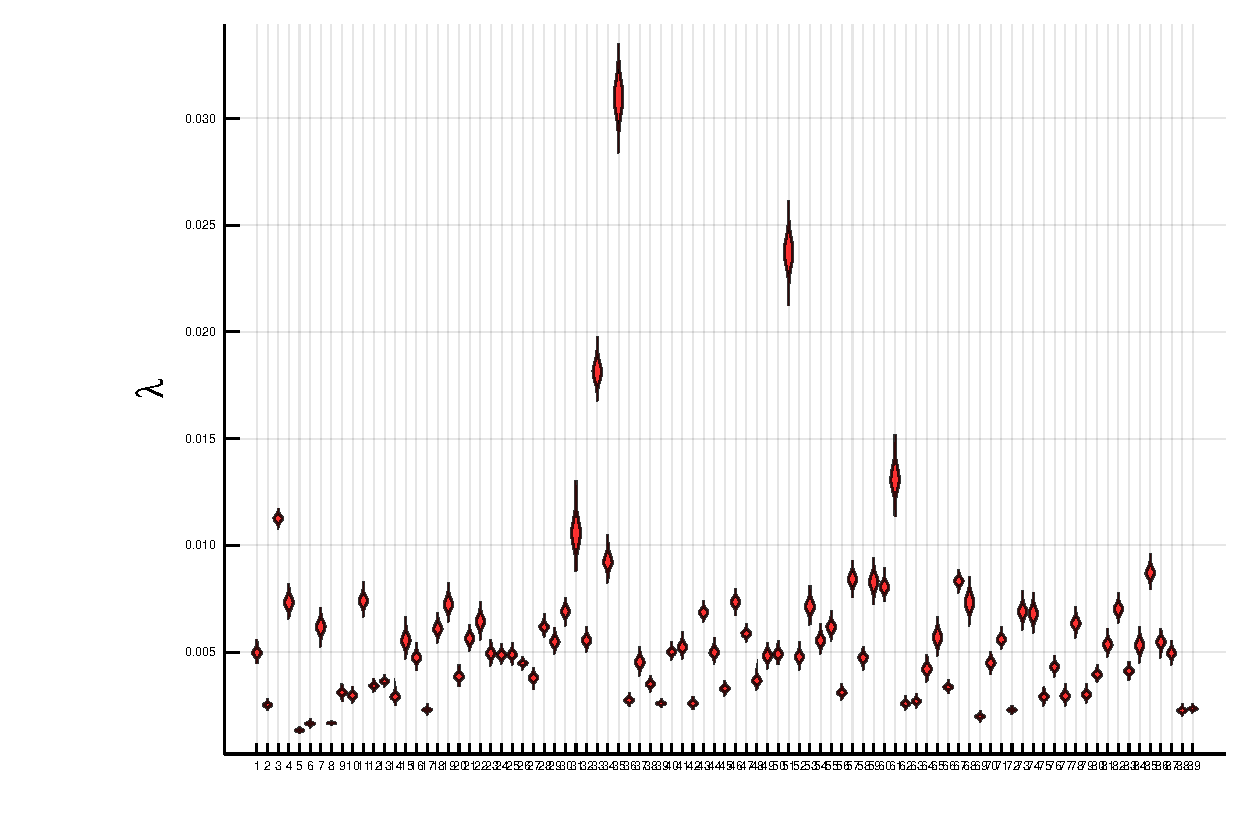
\includegraphics[width=7in]{images/PLAZA/plaza-lambda.pdf}
	}
	\caption[PLAZA Beluga duplication rates]{Overview of violin plots of the duplication rates $\lambda$ in each branch for the Beluga analysis of the PLAZA dataset.}
    \label{fig:plaza-lambda}
\end{figure}

\begin{figure}
    \noindent\makebox[\textwidth]{
        \hspace{-2.6cm}
	    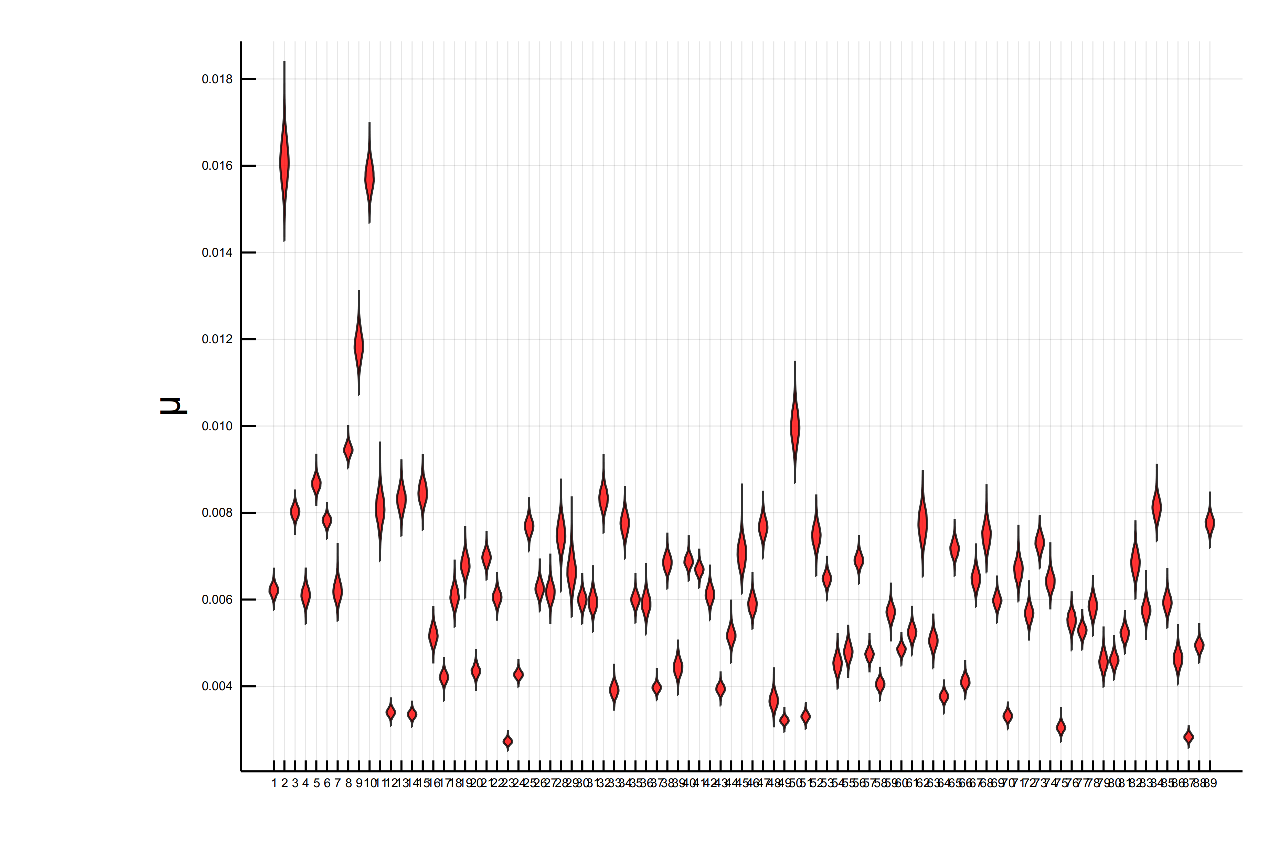
\includegraphics[width=7in]{images/PLAZA/plaza-mu.eps}
	}
	\caption[PLAZA Beluga loss rates]{Overview of violin plots of the loss rates $\mu$ in each branch for the Beluga analysis of the PLAZA dataset.}
    \label{fig:plaza-mu}
\end{figure}

\par We notice that the duplication rates (Figure \ref{fig:plaza-lambda}) and loss rates (Figure \ref{fig:plaza-mu}) are incredibly small, and there are very few outliers. Presumably this is because the branches in this species tree are, on average, much shorter than those in the smaller species trees; there is less time for events to occur. Also note that $\eta$ is tightly clustered around 0.5 in this result, so we do not have a situation where $\eta$ collapsed to zero which can sometime occur and usually indicates a faulty prior. It is unclear whether this is an abnormal result for this dataset, and should be an item for further study.

\begin{figure}
\begin{subfigure}{.5\textwidth}
  \centering
  \includegraphics[width=0.95\linewidth]{images/trees/plaza-tree.png}
  \caption{}
  \label{fig:sfig1}
\end{subfigure}%
\begin{subfigure}{.5\textwidth}
  \centering
  \includegraphics[width=0.95\linewidth]{images/trees/plaza-tree-2.png}
  \caption{}
  \label{fig:sfig2}
\end{subfigure}
\caption[Species tree of 44 PLAZA species]{Visualisations of the species tree used in the PLAZA experiment (44 species). Both the species tree with correct branch lengths (a) and a more visually clean tree with non-realistic branch lengths (b) are given. Trees were generated with iTOL \parencite{itol}.}
\label{fig:PLAZA-trees}
\end{figure}


\subsection{General notes on Beluga results}

The stochastic nature of the VI algorithms makes results strongly dependent on the initial parameter values of the variational distribution. When working on real-world data we observed that the starting values for the variational parameters must be chosen carefully and require some basic knowledge of the statistical model. The step-size parameter choice is also highly dependent on the model. In general we recommend the ADAM optimiser \parencite{ADAM} with a starting learning rate of 0.05. This learning rate should be lowered if excessive variability in the ELBO is noticed during the optimisation.
\\
We recommend the subsampling of the data into mini-batches of 100 to 200 samples since using smaller batches proved too noisy on real-world data. Conversely, using the full dataset on each iteration largely removes the speed advantage that VI has over the traditional MCMC methods.
\\
In general it appears that, of the two variational algorithms tested, BBVI is the most suitable for the Beluga model because it does not require calculation of the expensive model gradient. This means that we can use a much higher number of MC samples than ADVI and still converge faster.

\section{Whale model} \label{sec:whale}

\subsection{Introduction}
In this section we demonstrate another application of variational inference in a setting where previously only MCMC was used. The Whale library (see Methods and Materials) is another model currently in development at the VIB, and can be used to model hypothesised whole genome duplications (WGDs) in branches of the species tree \parencite{whale}. Whale uses probabilistic representations of gene trees (ALE) instead of the simple gene counts that are used in the Beluga model. As a result Whale is much slower; and a typical publishable analysis can take several days. This is an ideal candidate for variational inference because the improvement in computational speed could drastically change how analyses are performed.

\begin{figure}
	\centering
	\includegraphics[width=6.5in]{images/whale/whale-tree.png}
	\caption[Species tree of Whale experiment dataset]{Species tree used in the Whale experiment. Five hypothetical WGD nodes are placed on the species tree (black dots).}
    \label{fig:whale-tree}
\end{figure}


\subsection{Experiment}

\begin{figure}
	\centering
	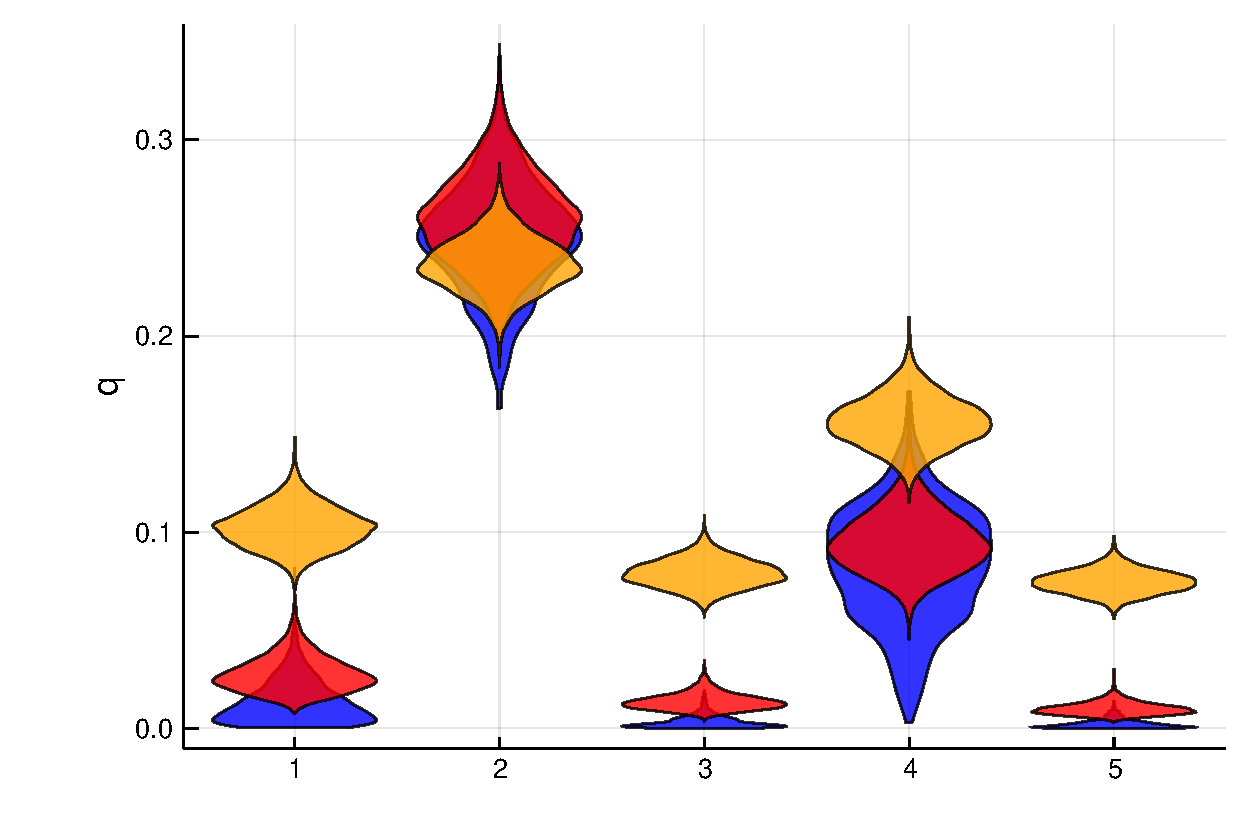
\includegraphics[width=5.2in]{images/whale/whale-q.pdf}
	\caption[Whale experiment retention rates $q$.]{Violin plots comparing the retention rates $q_i$ for the five hypothesised WGDs, with i$\, \in \{1, 5\}$. Plots are provided for the different methods of Bayesian inference: ADVI (yellow), BBVI (red) and MCMC (blue).}
    \label{fig:whale-q}
\end{figure}
\medskip
Just like the previously discussed Beluga model, Whale also models the evolutionary history of a set of species with duplication ($\lambda$) and loss rates ($\mu$), but here additional parameters $q$ are added, which model the retention of genes directly after a hypothesised WGD event.\footnote{Note that Beluga can also model whole genome duplications, we just chose not to in the previous examples.}
\medskip
\par We note that the variational methods ADVI and BBVI converge much faster here than the MCMC, which takes several hours even for a small dataset of only 500 samples. In comparison, the variational algorithms both converge in under 30 min and provide good approximations of the MCMC results.
\medskip
\par The BBVI results lead to the same conclusions as the MCMC regarding the presence of whole genome duplications in the evolutionary history of this species tree. We do not find evidence for a WGD in the branches of $q_1, \, q_3  \, or \, q_5$. There is, however, evidence for a WGD event in $q_2$. It is also evident that using ADVI here might lead to different conclusions, as ADVI finds more support a WGD in $q_4$ than the other methods.
All three methods find values closely centered around $\eta$=0.9.
\\
The resulting distributions for the duplication rates $\lambda$ and loss rates $\mu$ prove similar to the previous experiment with Beluga, in that both ADVI and BBVI give a very good approximation, but that BBVI appears on average to match MCMC slightly better.
\medskip
\par The variational solutions for the Whale are also affected by the initial parameter values.

\begin{figure}
	\centering
	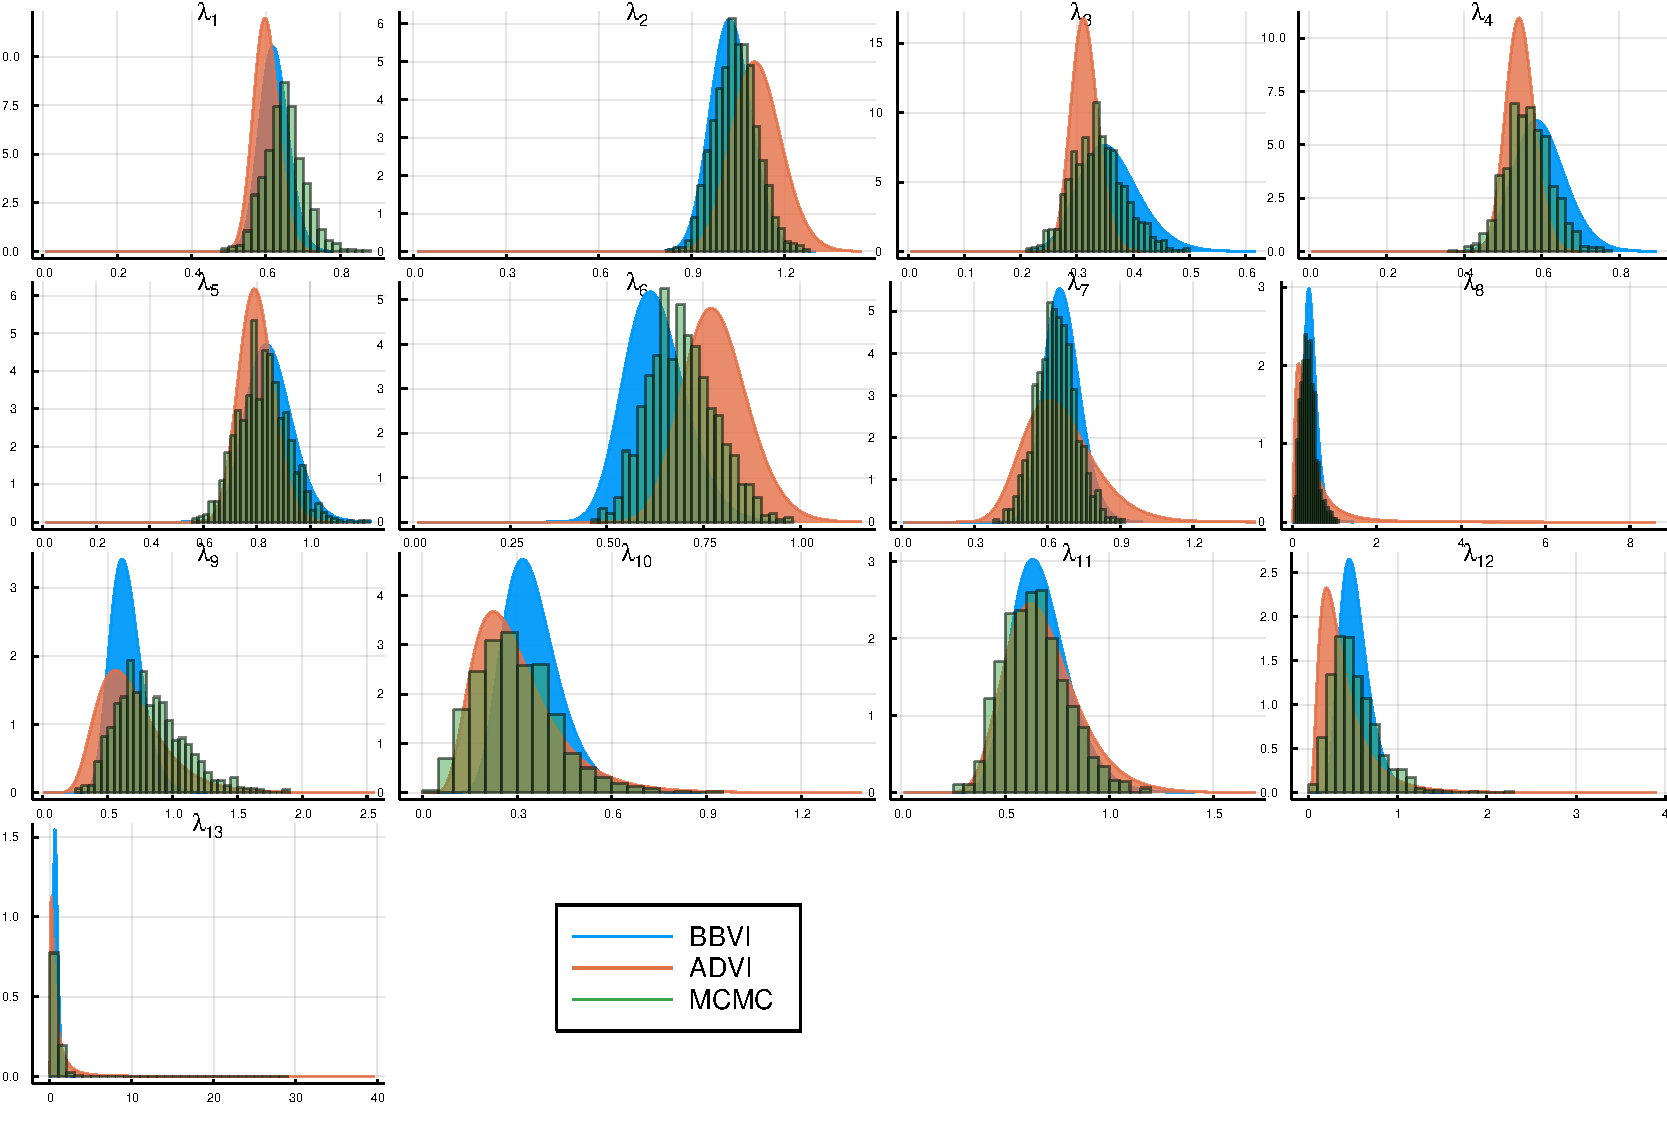
\includegraphics[width=6in]{images/whale/whale-distribution-lambda.pdf}
	\caption[Whale experiment $\lambda$ distributions.]{Comparison of different inference algorithms for the Whale model. The distributions of the different duplication rates $\lambda$ are given for BBVI (blue), ADVI (orange) and MCMC (green) respectively.}
    \label{fig:whale-lambda}
\end{figure}

\begin{figure}
	\centering
	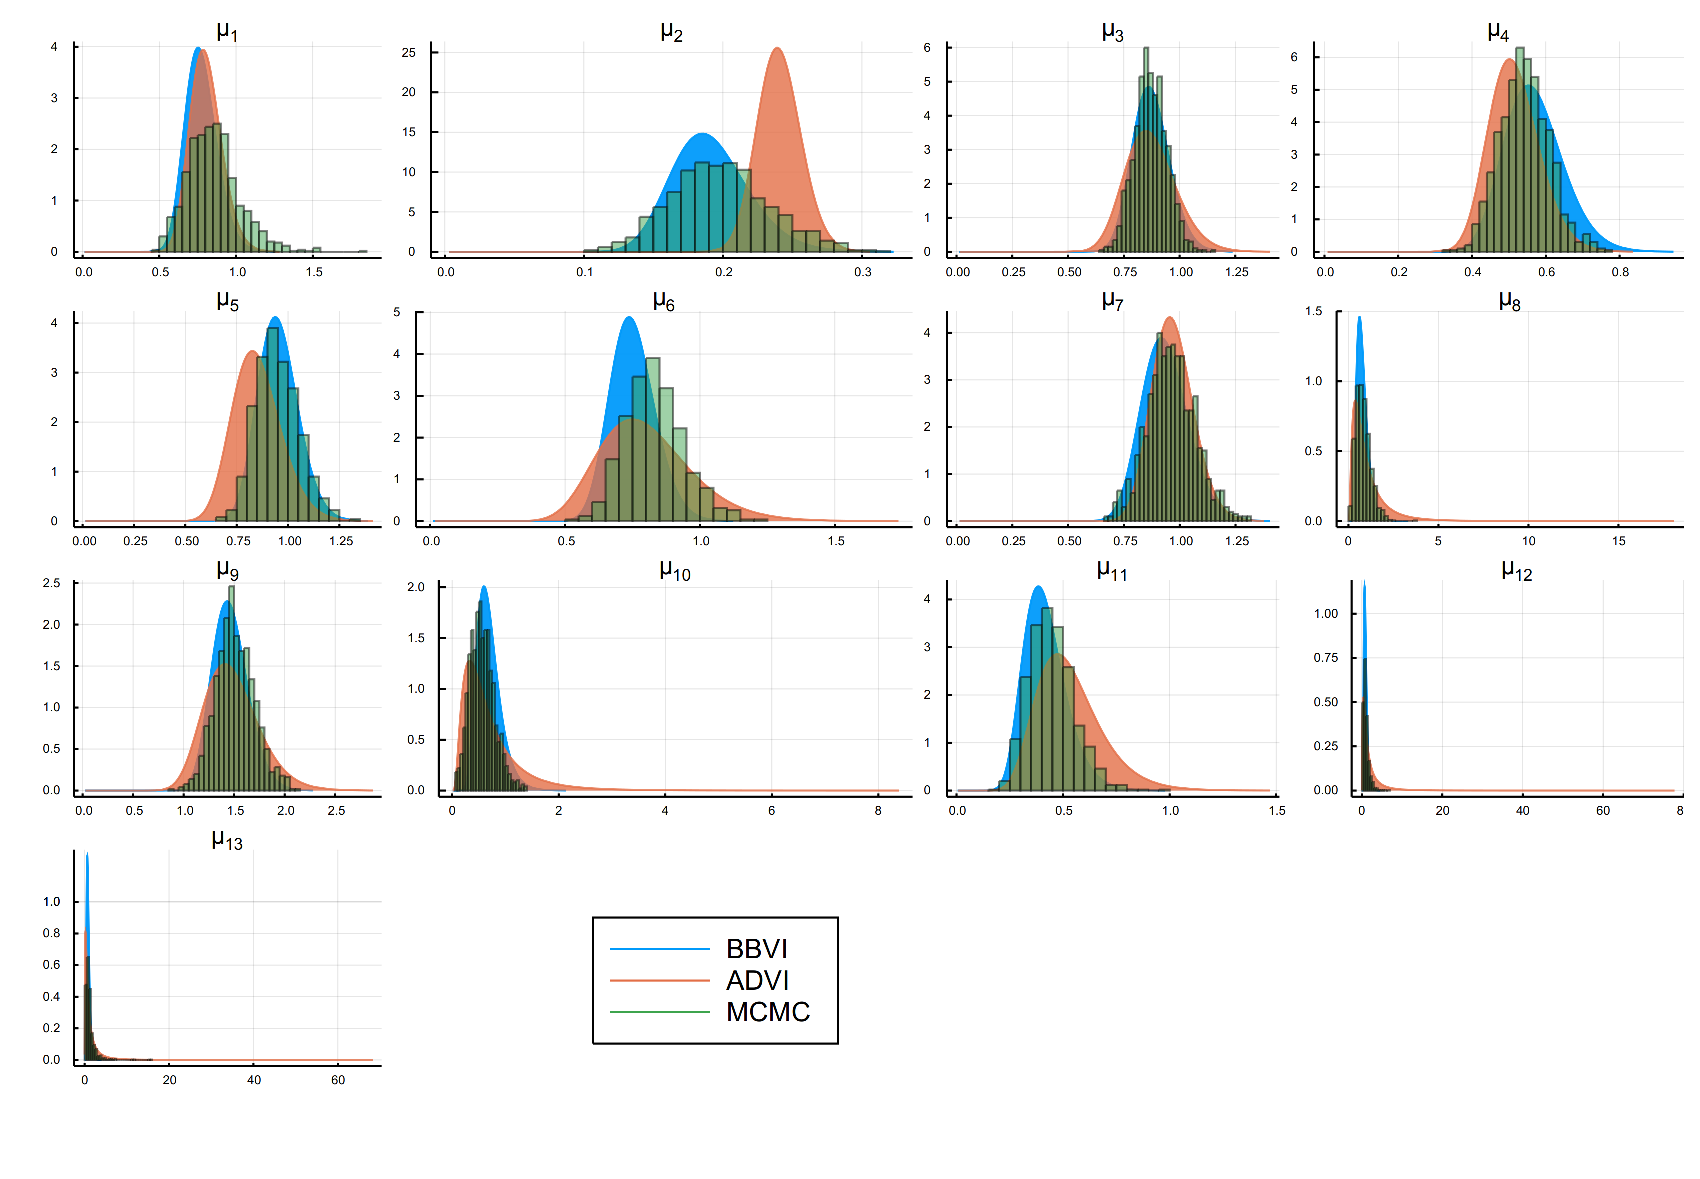
\includegraphics[width=6in]{images/whale/whale-distribution-mu.eps}
	\caption[Whale experiment $\mu$ distributions.]{Comparison of different inference algorithms for the Whale model. The distributions of the different loss rates $\mu$ are given for BBVI (blue), ADVI (orange) and MCMC (green) respectively.}
    \label{fig:whale-mu}
\end{figure}


\section{Conclusions}
In general it is clear from the experiments that the variational approximations can serve as a substitute for MCMC in cases where computational speed is preferred or where researcher want to design studies with larger species trees. For the Beluga and Whale models discussed in this Chapter, BBVI is both the fastest and most similar to MCMC of the variational algorithms that were studied.